\documentclass{standalone}
\usepackage{tikz}

\begin{document}

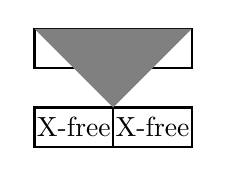
\begin{tikzpicture}[scale=1]
    % Draw the sub-counterwall G'
    \draw[black, thick] (0,0) rectangle (2,0.5);
    \node at (1,0.25) {\(G'\)};
    
    % Draw the first X-free brick
    \draw[black, thick] (0,-1) rectangle (1,-0.5);
    
    % Draw the second X-free brick
    \draw[black, thick] (1,-1) rectangle (2,-0.5);
    
    % Draw the triangle representing the section
    \fill[gray] (0,0.5) -- (1,-0.5) -- (2,0.5) -- cycle;
    
    % Labeling the top row of bricks
    \node at (0.5,-0.75) {X-free};
    \node at (1.5,-0.75) {X-free};
\end{tikzpicture}

\end{document}